% LuaTeX Project Setup and Compilation Guide

% This document outlines the necessary steps to configure a comprehensive LaTeX environment 
% for editing and typesetting documents using either Emacs with AUCTeX or the Kile editor.

%----------------------------------------------------------------------------------------
% 1. Installing a TeX Distribution

% Choose one of the following TeX distributions based on your operating system:

% Linux:
%   TeX Live:*Recommended for its extensive package collection and regular updates.
%     ```bash
%     sudo dnf install texlive-full  % Comprehensive installation
%     sudo dnf install texlive-babel-russian  % Russian language support
%     ```
%   Other Distributions:*Explore options like TeX Live or TeXstudio depending on your preferences.
% Windows:
%   MiKTeX:*A popular choice with on-the-fly package installation. Download the installer from https://miktex.org/download.
% macOS:
%   MacTeX:*A complete TeX distribution specifically for macOS. Download from https://tug.org/mactex/.

%----------------------------------------------------------------------------------------
% 2. Essential LaTeX Packages

% Install the following packages using your TeX distribution's package manager (e.g., `tlmgr` for TeX Live):

% fontspec:*Advanced font selection and OpenType font support.
% enumitem:*Customization of list environments.
% extsizes:*Extended font size options. 
% subfig:*Management of subfigures and captions.
% caption:*Enhanced caption formatting.
% natbib:*Flexible bibliography management.
% babel-russian:*Russian language hyphenation and typography support.
% titlesec:*Customization of section headings.
% lh:*Cyrillic font support for LuaLaTeX or XeLaTeX.

%----------------------------------------------------------------------------------------
% 3. Editor Configuration

% Select your preferred LaTeX editor:

% Doom Emacs
%   1. Install latex for doomemacs: Refer to the Emacs package manager or official instructions - https://docs.doomemacs.org/v21.12/modules/lang/latex/.
%   2. Optionally, install and configure `pdf-tools` for enhanced PDF interaction within Emacs. 
% Kile:
%   1. Install Kile using your system's package manager or download from https://kile.org/.
%   2. Kile provides a user-friendly graphical interface with project management, syntax highlighting, 
%      code completion, and integrated PDF viewing.

%----------------------------------------------------------------------------------------
% 4. Compilation and Workflow

% Use the appropriate command or keybinding to compile your LaTeX document (e.g., `pdflatex` for PDF output).
% Configure your editor to automatically build and view the generated PDF.
% Utilize the features of your chosen editor and installed packages to enhance your LaTeX workflow.

%----------------------------------------------------------------------------------------
% 5. Additional Resources

% Comprehensive TeX documentation: https://www.tug.org/texlive/doc.html
% LaTeX community forums and support: https://tex.stackexchange.com/
% Package documentation and examples: Refer to the respective package websites or CTAN (https://ctan.org/).

%----------------------------------------------------------------------------------------

\documentclass[12pt, a4paper]{extreport}

\usepackage[english, russian]{babel}
\usepackage{fontspec} % Advanced font management
\usepackage{graphicx}
\usepackage[margin=2.5cm]{geometry} % Consistent margins
\usepackage{titlesec} % Customize section headings
\usepackage{fancyhdr} % Customize headers and footers
\usepackage{enumitem}
\usepackage{subfig}
\usepackage{hyperref}
\usepackage{authblk}
\usepackage{titling}
\usepackage[numbers]{natbib}

\hypersetup{
  colorlinks=false, 
}

\title{МЕТОДЫ ОЦЕНКИ ВЛИЯНИЯ КОСМИЧЕСКОЙ ПОГОДЫ НА БОРТОВЫЕ СИСТЕМЫ НИЗКООРБИТАЛЬНЫХ СПУТНИКОВ}
\author{Глеба Е. М., Баранова В. С.}
\date{\the\year}

\graphicspath{{img/}}

\setmainfont[Path = ./fonts/,
             UprightFont = *-Regular,
             BoldFont = *-Bold,
             ItalicFont = *-Italic,
             BoldItalicFont = *-BoldItalic]{Times New Roman}

\titleformat*{\section}{\Large\bfseries}
\titleformat*{\subsection}{\large\bfseries}

% Set up headers and footers
\pagestyle{fancy}
\fancyhf{} % Clear default headers and footers
\fancyhead[C]{\textbf{Методы оценки влияния космической погоды}} % Centered header
\fancyfoot[C]{\thepage} % Page number in footer

\renewcommand{\thesection}{\arabic{section}} 

\begin{document}

\begin{titlepage}
    \begin{center}
        \Large \textbf{МИНИСТЕРСТВО ОБРАЗОВАНИЯ РЕСПУБЛИКИ БЕЛАРУСЬ БЕЛОРУССКИЙ ГОСУДАРСТВЕННЫЙ УНИВЕРСИТЕТ
            ФАКУЛЬТЕТ РАДИОФИЗИКИ И КОМПЬЮТЕРНЫХ ТЕХНОЛОГИЙ
        } \\
        Кафедра физики и аэрокосмических технологий
    \end{center}

    \vspace{5em}

    \begin{center}
        \Huge \textsc{\textbf{Курсовая работа}}
    \end{center}

    \begin{center}
        \Large \thetitle
    \end{center}

    \vspace{2em}

    \hfill
    \parbox{14em}{
        Глеба Евгения Михайловича \\
        студента 3 курса, \\
        специальность «аэрокосмические \\
        радиоэлектронные и информационные \\
        системы и технологии» \\
        \\
        Научный руководитель: \\
        Баранова Василина Сергеевна \\
    }


    \begin{center}
        Минск, \thedate
    \end{center}

\end{titlepage}

\tableofcontents

\newpage

\section{Введение}

Космическая погода представляет собой комплекс явлений, происходящих в околоземном космическом пространстве, которые могут влиять на работу низкоорбитальных спутников. К ним относятся: солнечные вспышки, выбросы корональной массы, геомагнитные бури. Влияние космической погоды может проявляться в виде аномалий телеметрии, сбоев в работе бортовых систем и даже полной потери спутника \cite{green2017impact}. В большинстве случаев, для обнаружения аномалий используются критерии на основе пороговых значений нижних и верхних пределов наиболее критичных параметров телеметрии бортовой электроники наноспутника. Также в последнее время, в область проектирования и эксплуатации наноспутников внедряются автоматизированные системы мониторинга состояния телеметрии, которые используют различные модели машинного обучения \cite{schlag2018numerical}. Подобные автоматизированные системы оценивают в целом работоспособность бортовых систем на момент испытаний или в режиме полетной диагностики. Спутник является сложной электрической системой, где события на каждом узле (компоненты бортовых систем) могу привести к последовательности не предугаданных сбоев. Причиной сбоев может послужить как естественные неполадки бортовых компонентов, так и внешние факторы.  В данной работе проводится оценка взаимосвязи и влияния солнечной активности на работу бортовой электроники по данным телеметрии космических аппаратов, а также разработка и оптимизация готовых решений с открытым исходным кодом для анализа больших данных.

\newpage

\section{SatNOGS: Открытая инфраструктура для мониторинга низкоорбитальных спутников}

SatNOGS представляет собой комплексную платформу, обеспечивающую функционирование открытой сети наземных станций для мониторинга спутников. Основной целью проекта является разработка полного стека открытых технологий, основанных на открытых стандартах, и создание полноценной наземной станции в качестве демонстрации возможностей данного стека. Система SatNOGS способна принимать сигналы со спутников, находящихся на низкой околоземной орбите (LEO), в диапазонах UHF и VHF. Она позволяет извлекать сигналы состояния и телеметрии, данные с научных и исследовательских спутников (например, результаты магнитосферных экспериментов), метеорологические данные и другую информацию.

\subsection{Истоки и Технологии}

Проект SatNOGS зародился в 2014 году во время мероприятия NASA SpaceApps Hackathon, проходившего в Афинском хакерспейсе. Он предоставляет набор технологий, необходимых для создания распределенной сети наземных станций, предназначенных для наблюдения за спутниками на низкой околоземной орбите.
Ключевыми компонентами SatNOGS являются:

\begin{itemize}[label=\textbullet]
    \item	SatNOGS Network: Веб-приложение, предназначенное для планирования наблюдений по сети наземных станций. Оно способствует координации наблюдений за спутниковыми сигналами и планированию таких наблюдений среди наземных станций, подключенных к сети.
    \item	База данных SatNOGS: Ресурс, позволяющий пользователям предоставлять информацию о передатчиках активных спутников. Данные доступны через API или веб-интерфейс.
    \item	Клиент SatNOGS: Программное обеспечение, работающее на наземных станциях (обычно на встраиваемых системах). Оно получает регулярные задания на наблюдение из сети, принимает спутниковые передачи и отправляет их обратно в веб-приложение Network.
    \item	Наземная станция SatNOGS: Аппаратное обеспечение наземной станции с открытым исходным кодом, включающее ротаторы, антенны и электронику, подключенные к клиенту.
\end{itemize}

\subsection{Функционал и Применение}

SatNOGS фокусируется на приеме данных со спутников, а не на отправке команд. Спутники обычно передают телеметрические данные практически непрерывно, что позволяет операторам и другим пользователям сети SatNOGS получать, декодировать и ретранслировать эту информацию.
Одной из ключевых задач проекта является стимулирование разработчиков спутников (особенно создателей CubeSat) к использованию протоколов с открытым исходным кодом для передачи данных. Это обеспечивает дополнительную возможность декодирования таких протоколов системой SatNOGS и сбор телеметрической информации с множества различных наземных станций.

\subsection{Преимущества Открытости}

SatNOGS реализует концепцию массового строительства и развертывания любительских станций слежения по всему миру, основанных на технологиях с открытым исходным кодом и открытых стандартах. Такой подход обеспечивает:

\begin{itemize}[label=\textbullet]
    \item	Модульность: Система легко модифицируется и адаптируется к различным задачам.
    \item	Автономность: Станции подключаются к интернету и работают полностью автоматически.
    \item	Доступность: Открытый исходный код и стандарты способствуют широкому распространению и развитию технологий.
\end{itemize}

В целом, SatNOGS представляет собой мощный инструмент для мониторинга низкоорбитальных спутников, способствующий развитию открытой космической инфраструктуры.

\newpage

\section{Платформа Polaris ML}

Платформа Polaris ML. Приложение Polaris ML от LibreSpace использует алгоритм машинного обучения XGBoost для анализа взаимосвязей между параметрами телеметрии бортовых систем спутника. Polaris ML способен рассчитать и визуализировать взаимосвязи между параметрами телеметрии и степень их влияния друг на друга в виде трехмерного графа связностей. В процессе исследования производительность модели искусственного интеллекта Polaris ML была значительно усовершенствована путем переноса core инфраструктуры на C++, а именно выделением прекомпилированных библиотек ввода/вывода и кэширования промежуточных расчетов обучения. Также в приложение Polaris были добавлены декодеры для отслеживания целевых спутников и модуль, собирающий информацию о солнечной активности, работающий в отдельном контейнере Docker. Кроме того, был доработан инструмент для построения графов связностей и веб-интерфейс. Внедрены решения для прямого взаимодействия с панелью управления сервера SatNOGS, что позволяет получать дополнительные данные о состоянии интересующих спутников.
На рис. \ref{fig:polaris_architecture} представлена архитектура финальной системы, включающая в себя внесенные доработки и усовершенствования.

\begin{figure}[htbp]
    \centering
    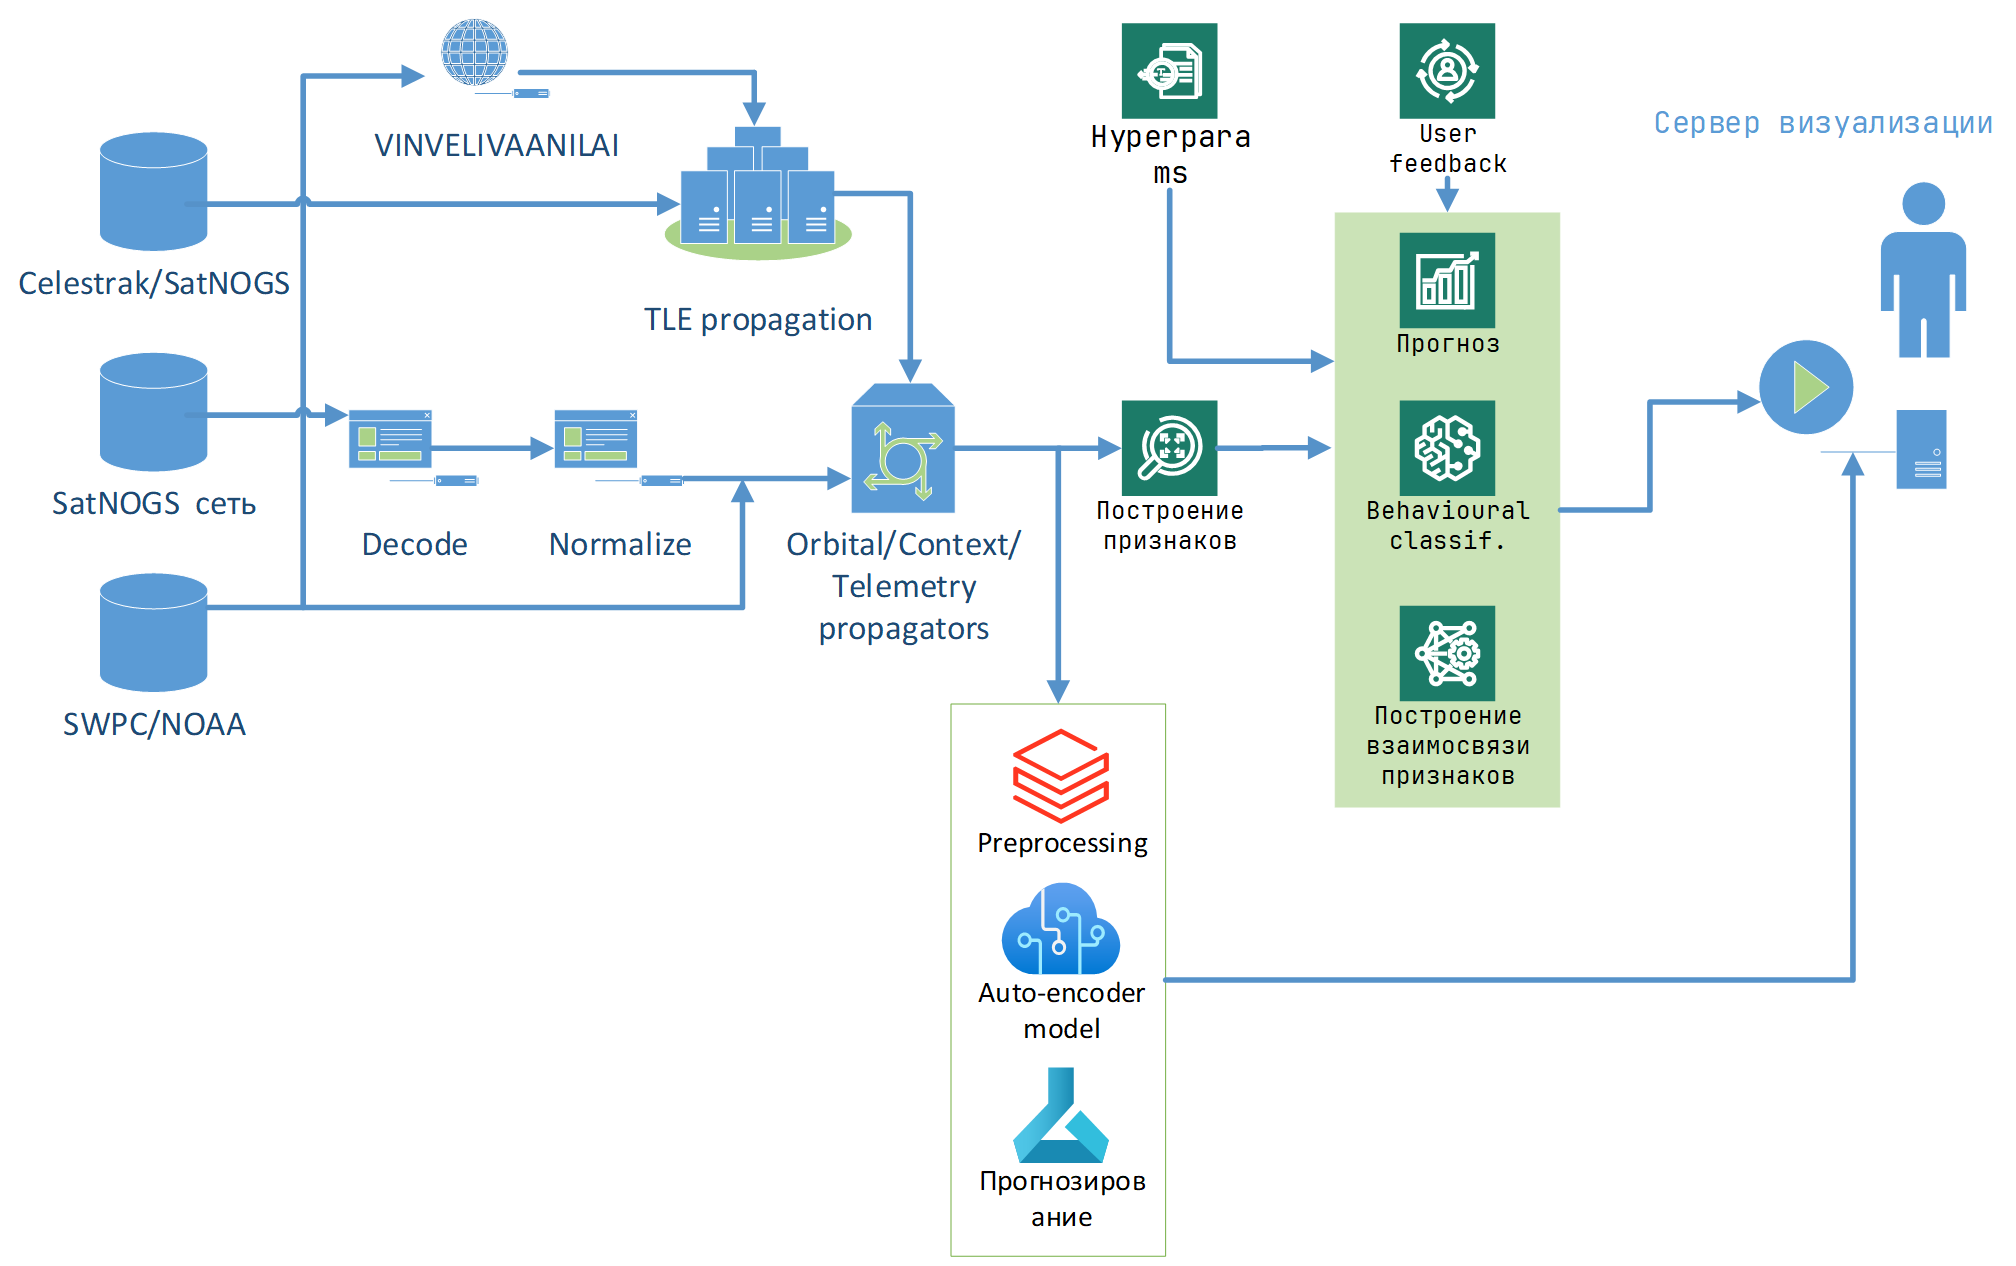
\includegraphics[width=0.8\textwidth]{polaris_architecture.png}
    \caption{Архитектура приложения Polaris}
    \label{fig:polaris_architecture}
\end{figure}

Этапы проведения анализа: 

\begin{enumerate}[label=\arabic*.]
\item \textbf{Автоматическое извлечение данных:} 
    Данные извлекаются из различных источников, включая телеметрию сети SatNOGS и данные о космической погоде от NASA SWPC (NOAA).

\item \textbf{Машинное обучение (XGBoost):}
    С использованием алгоритма XGBoost \cite{xgboost}\cite{boumghar2018enhanced} анализируется взаимосвязь извлеченных данных. Результатом является файл в формате JSON, содержащий описания параметров телеметрии и их значения в кадрах с временными метками.

\item \textbf{Визуализация:} 
    Строится граф связности для визуализации взаимозависимостей между параметрами. Также создается сложенный нормализованный вид телеметрии для отображения аномалий.

\item \textbf{Экспорт данных:} 
    Выходные данные графиков экспортируются для дальнейшего анализа и интерпретации.
\end{enumerate}

Как упоминалось ранее, был создан дополнительный модуль, который извлекает информацию о космической погоде с серверов NASA SWPC/NOAA. Эти данные сохраняются в базу данных InfluxDB, которая развернута локально в отдельном контейнере Docker Compose. Модуль также оснащен функциями для анализа данных орбитальных параметров в форматах TLE и OMM, а также для прогнозирования движения спутников на основе этих данных \cite{bottou1991stochastic}\cite{killick2012optimal}.

Анализ перезагрузок основного процессор и граф связности. На рис.\ref{fig:grifex_resets_vs_solar_params} представлена взаимосвязь количества перезагрузок основного процессора наноспутника формата 3U GRIFEX от следующих индексов солнечной активности за период с 2019-03-03 по 2024-02-22: среднемесячные значения пятен S.I.D.C., SWPC/SWO и f10.7 см радиоизлучение. На рис.\ref{fig:grifex_graph} представлен результат использования модели Polaris ML для построения 3D графа связности параметров телеметрии спутника GRIFEX за период 2015–2021 г.

\begin{figure}[htbp]
    \centering
    \subfloat[]{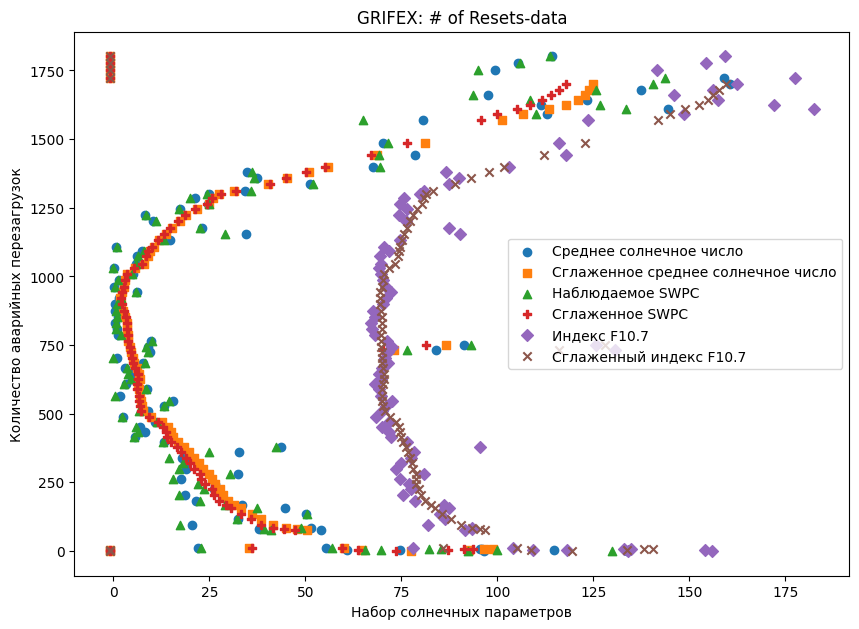
\includegraphics[width=0.65\textwidth]{grifex_resets_vs_solar_params.png}\label{fig:grifex_resets_vs_solar_params}}
    \hfill % Adds horizontal space between the images
    \subfloat[]{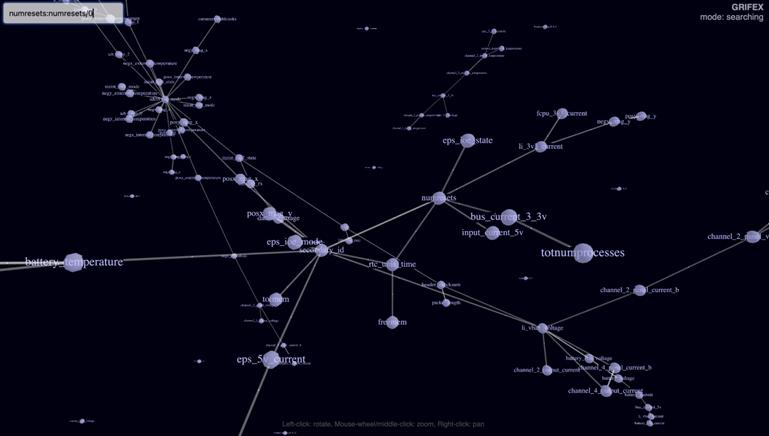
\includegraphics[width=0.75\textwidth]{grifex_graph.png}\label{fig:grifex_graph}}
    \caption{(\ref{fig:grifex_resets_vs_solar_params}) - диаграмма количества принудительных перезагрузок основного процессора с набором параметров активности Солнца для спутника GRIFEX; (\ref{fig:grifex_graph}) - 3D граф связности параметров телеметрии спутника GRIFEX}
    \label{fig:combined_figure}
\end{figure}

Как видно, количество перезагрузок основного процессора GRIFEX стремительно накапливалось в период 2019–2020 г., когда индексы солнечной активности SWPC/SWO и f10.7 см были относительно постоянны. С 2020 начался новый 5-летний цикл солнечной активности, что соответствуют замедлению роста количества перезагрузок. Причина такого поведения объясняется графом связности. Из анализа графа видно, все взаимозависимые параметры телеметрии образуют
взаимосвязанные ветки относительно времени (rtc\_unix\_time), а также относительно критичных параметров. Общее количество перезагрузок основного процессора (numresets) непосредственно связанно с токовым потреблением в бортовой системе питания, в частности, с значением тока на общей шине питания (battery\_bus\_current), с уровнем тока на шине 3.3 В (bus\_current\_3\_3v), с уровнем тока на шине 3.3 В основного процессора (fcpu\_3v3\_current), с уровне тока на шине 3.3 В аккумулятора (li\_3v3\_current).
Из графа также видно, что на количество перезагрузок процессора влияет число запущенных процессов (totnumprocesses). Можно предположить, что количество перезагрузок связанно с просадкой напряжения на шине питания за счет низкой температуры на аккумуляторах (battery\_temperature). При увеличении солнечной активности увеличился общий световой поток, что привело к повышению температуры, стабилизации напряжения и несвойственному замедлению роста числа перезагрузок процессора.

Таким образом, доработанная и адаптированная модель Polaris ML может быть использована для комплексного анализа взаимосвязей и влияния различных факторов на работу бортовой электроники наноспутников, в частности, солнечной активности. Оценка большего объема данных позволит выявить наиболее уязвимые системы спутника для разработки безопасных режимов работы его бортового оборудования в условиях агрессивной солнечной активности.

\section{Алгоритм XGBoost}

\begin{enumerate}[label=\arabic*.]
\item \textbf{Инициализация модели:} 
  Определяется начальная модель $F_0(x)$ как константа, минимизирующая функцию потерь на обучающей выборке:

  $$F_0(x) = \arg \min_{\gamma} \sum_{i=1}^n L(y_i, \gamma)$$

\item \textbf{Итеративное построение ансамбля:} 
  Процесс построения модели происходит итеративно, добавляя по одному дереву за раз:
    \begin{enumerate}[label=\roman*.]
        \item \textbf{Вычисление градиентов и значений функции потерь:} Для каждого объекта в обучающей выборке вычисляются градиент ($g_i$) и значение функции потерь ($h_i$):

            $$g_i = \frac{\partial L(y_i, F_{m-1}(x_i))}{\partial F_{m-1}(x_i)}$$

            $$h_i = \frac{\partial^2 L(y_i, F_{m-1}(x_i))}{\partial F_{m-1}(x_i)^2}$$

        \item \textbf{Построение дерева решений:} Строится дерево решений $f_m(x)$, минимизирующее функцию потерь с учетом регуляризации:

            $$\mathcal{L}^{(m)} = \sum_{i=1}^n \left[ g_i f_m(x_i) + \frac{1}{2} h_i f_m^2(x_i) \right] + \Omega(f_m)$$

            где $\Omega(f_m)$ - функция регуляризации, контролирующая сложность дерева.

        \item \textbf{Обновление модели:} Модель обновляется путем добавления нового дерева с весом, определяемым коэффициентом обучения $\alpha_m$:

            $$F_m(x) = F_{m-1}(x) + \alpha_m f_m(x)$$
    \end{enumerate}

\item \textbf{Предсказание:} 
  Для нового объекта $x$ предсказание модели получается суммированием предсказаний всех деревьев:

  $$\hat{y} = F_M(x) = \sum_{m=1}^M \alpha_m f_m(x)$$
\end{enumerate}

Особенности XGBoost:

\begin{itemize}
\item \textbf{Регуляризация:} Предотвращает переобучение и повышает обобщающую способность модели.
\item \textbf{Метод Ньютона-Рафсона:} Используется для эффективной оптимизации функции потерь.
\item \textbf{Обработка разреженных данных:} XGBoost эффективно работает с разреженными данными, что важно для многих задач.
\item \textbf{Параллельное вычисление:} Алгоритм поддерживает параллельное вычисление для ускорения обучения.
\end{itemize}

\section{Polaris ML: Выявление аномалий в данных телеметрии}

Polaris ML, разработанная Libre Space Foundation, представляет собой мощную платформу для анализа данных телеметрии спутников. В основе платформы лежит алгоритм XGBoost, позволяющий выявлять аномалии и строить графы связности, отражающие взаимозависимости параметров телеметрии. 

\subsection{Процесс анализа}

\begin{enumerate}[label=\arabic*.]
\item \textbf{Извлечение фреймов:} Процесс анализа начинается с сегментации временного ряда телеметрии на фреймы. Это может быть выполнено с фиксированным размером окна или на основе определенных событий.
\item \textbf{Извлечение признаков:} Из каждого фрейма извлекаются разнообразные статистические характеристики, такие как среднее значение, стандартное отклонение, минимум, максимум и другие, формируя вектор признаков.
\item \textbf{Обучение модели XGBoost:} Модель XGBoost обучается на основе векторов признаков, полученных из фреймов. Цель - создать модель, способную предсказывать значения параметров телеметрии в будущих фреймах.
\item \textbf{Выявление аномалий:} Аномалии определяются как значительные отклонения от предсказанных моделью XGBoost значений. Для этого Polaris ML предлагает несколько подходов:
    \begin{enumerate}[label=\alph*.]
        \item \textbf{Пороговые значения:} Устанавливаются пределы отклонений от предсказанных значений, например:

        $$\| y_i - \hat{y}_i \| > \epsilon$$

        где $y_i$ - реальное значение, $\hat{y}_i$ - предсказанное значение, а $\epsilon$ - заданный порог.
        \item \textbf{Статистические методы:} Используются z-оценка:

        $$z_i = \frac{y_i - \mu}{\sigma}$$

        где $\mu$ - среднее значение, $\sigma$ - стандартное отклонение, и тест Граббса:

        $$G = \frac{\max_{i}|y_i - \bar{y}|}{s}$$

        где $\bar{y}$ - выборочное среднее, $s$ - выборочное стандартное отклонение, для выявления выбросов.
    \end{enumerate}
\item \textbf{Графы связности:} Модель XGBoost также используется для построения графов связности, визуализирующих взаимосвязи между параметрами телеметрии. Это помогает анализировать влияние изменений одних параметров на другие и выявлять потенциальные причины аномалий.
\end{enumerate}

\subsection{Расширенный инструментарий}

Помимо XGBoost, Polaris ML может использовать и другие методы выявления аномалий, включая:

Методы, основанные на расстоянии: Евклидово расстояние, Манхэттенское расстояние, расстояние Махаланобиса.
Методы, основанные на плотности: Local Outlier Factor (LOF), Isolation Forest.
Методы машинного обучения: One-Class SVM, автоэнкодеры.

Выбор конкретных методов зависит от характеристик данных и целей анализа.

\newpage 

\begin{thebibliography}{99}

    \bibitem{green2017impact}
    Green, J. C., Likar, J., \& Shprits, Y. (2017). Impact of space weather on the satellite industry. \textit{Advancing Earth and space science}, 15, 804--818.

    \bibitem{schlag2018numerical}
    Schlag, L., O'Meara, C., \& Wickler, M. (2018). Numerical Analysis of Automated Anomaly Detection Algorithms for Satellite Telemetry. In \textit{SpaceOps Conference} (pp. 1-13).

    \bibitem{xgboost}
    XGBoost: A Scalable Tree Boosting System [Электронный ресурс]. Retrieved March 7, 2024, from https://xgboost.readthedocs.io/en/latest/

    \bibitem{boumghar2018enhanced}
    Boumghar, R., Silva, J., Angelis, I., Schulster, J., \& Donati, A. (2018). Enhanced awareness in space operations using multipurpose dynamic network analysis. In \textit{Space Operations: Inspiring Humankind's Future} (pp. 795-810). Springer International Publishing.

    \bibitem{ray2002bayesian}
    Ray, B. K., \& Tsay, R. S. (2002). Bayesian methods for changepoint detection in long-range dependent processes. \textit{Journal of Time Series Analysis}, 23, 687--705.

    \bibitem{bottou1991stochastic}
    Bottou, L. (1991). Stochastic gradient learning in neural networks. In \textit{Proceedings of Neuro-Nimes} (Vol. 91).

    \bibitem{killick2012optimal}
    Killick, R., Fearnhead, P., \& Eckley, I. A. (2012). Optimal detection of changepoints with a linear computational cost. \textit{J. Amer. Statist. Assoc.}, 107, 1590--1598.

\end{thebibliography}

\end{document}
